\documentclass[12pt, oneside]{article}

\usepackage[letterpaper, scale=0.8, centering]{geometry}
\usepackage{fancyhdr}
\setlength{\parindent}{0em}
\setlength{\parskip}{1em}

\pagestyle{fancy}
\fancyhf{}
\renewcommand{\headrulewidth}{0pt}
\rfoot{{\footnotesize Copyright Mia Minnes, 2025, Version \today~(\thepage)}}

\usepackage{titlesec}

\author{CSE105W25}

\newcommand{\instructions}{{\bf For all HW assignments:} Weekly homework 
may be done individually or in groups of up to 3 students. 
You may switch HW partners for different HW assignments. 
Please ensure your name(s) and PID(s) are clearly visible on the first page of your homework submission 
and then upload the PDF to Gradescope. If working in a group, submit only one submission per group: 
one partner uploads the submission through their Gradescope account and then adds the other group member(s) 
to the Gradescope submission by selecting their name(s) in the ``Add Group Members" dialog box. 
You will need to re-add your group member(s) every time you resubmit a new version of your assignment.
 Each homework question will be graded either for correctness (including clear and precise explanations and 
 justifications of all answers) or fair effort completeness. 
 On the ``graded for correctness"
 questions, you may only collaborate with CSE 105 students in your group; if your
 group has questions about a problem, you may ask in drop-in help hours or post a private
post (visible only to the Instructors) on Piazza. On the "graded for completeness" questions, you 
may collaborate with all other CSE 105 students this quarter, and you may make public posts about these questions 
on Piazza.

All submitted homework for this class must be typed. 
You can use a word processing editor if you like (Microsoft Word, Open Office, Notepad, Vim, Google Docs, etc.) 
but you might find it useful to take this opportunity to learn LaTeX. 
LaTeX is a markup language used widely in computer science and mathematics. 
The homework assignments are typed using LaTeX and you can use the source files 
as templates for typesetting your solutions.
To generate state diagrams of machines, you can (1) use the LaTex tikzpicture
environment (see templates in the class notes), or (2) use the software tools Flap.js or
JFLAP described in the class syllabus (and include a screenshot in your PDF), or (3) you can carefully
and clearly hand-draw
the diagram and take a picture and include it in your PDF.
We recommend that you
submit early drafts to Gradescope so that in case of any technical difficulties, at least some of your
work is present. You may update your submission as many times as you'd like up to the deadline.


{\bf Integrity reminders}
\begin{itemize}
\item Problems should be solved together, not divided up between the partners. The homework is
designed to give you practice with the main concepts and techniques of the course, 
while getting to know and learn from your classmates.
\item On the "graded for correctness"
questions, you may only collaborate with CSE 105 students in your group.
You may ask questions about the homework in office hours (of the instructor, TAs, and/or tutors) and 
on Piazza (as private notes viewable only to the Instructors).  
You \emph{cannot} use any online resources about the course content other than the class material 
from this quarter -- this is primarily to ensure that we all use consistent notation and
definitions (aligned with the textbook) and also to protect the learning experience you will have when
the `aha' moments of solving the problem authentically happen.
\item Do not share written solutions or partial solutions for homework with 
other students in the class who are not in your group. Doing so would dilute their learning 
experience and detract from their success in the class.
\end{itemize}

}

\newcommand{\gradeCorrect}{({\it Graded for correctness}) }
\newcommand{\gradeCorrectFirst}{\gradeCorrect\footnote{This means your solution 
will be evaluated not only on the correctness of your answers, but on your ability
to present your ideas clearly and logically. You should explain how you 
arrived at your conclusions, using
mathematically sound reasoning. Whether you use formal proof techniques or 
write a more informal argument
for why something is true, your answers should always be well-supported. 
Your goal should be to convince the
reader that your results and methods are sound.} }
\newcommand{\gradeComplete}{({\it Graded for completeness}) }
\newcommand{\gradeCompleteFirst}{\gradeComplete\footnote{This means you will 
get full credit so long as your submission demonstrates honest effort to 
answer the question. You will not be penalized for incorrect answers. 
To demonstrate your honest effort in answering the question, we 
expect you to include your attempt to answer *each* part of the question. 
If you get stuck with your attempt, you can still demonstrate 
your effort by explaining where you got stuck and what 
you did to try to get unstuck.} }

\usepackage{tikz}
\usetikzlibrary{automata,positioning,arrows}

\input{../../resources/discrete-math-packages}

\newcommand{\SUBSTRING}{\textsc{Substring}}
\newcommand{\REP}{\textsc{Rep}}
\newcommand{\blank}{\scalebox{1.5}{\textvisiblespace}}


\title{HW6CSE105F24: Homework assignment 6}
\date{Due: December 3, 2024 at 5pm, via Gradescope}


\begin{document}
\maketitle
\thispagestyle{fancy}

{\bf In this assignment,}

You will  practice analyzing, designing, and working with Turing machines.
You will use general constructions and specific machines to explore the classes 
of recognizable and decidable languages. 
You will explore various ways to encode machines as strings so that 
computational problems can be recognized.

{\bf Resources}: To review the topics 
for this assignment, see the class material from Weeks 8 and 9.
We will post frequently asked questions and our answers to them in a 
pinned Piazza post. 

{\bf Reading and extra practice problems}:  
Sipser Sections 4.2, 5.3, 5.1.
Chapter 4 exercises 4.9, 4.12.
Chapter 5 exercises 5.4, 5.5, 5.6, 5.7. 
Chapter 5 problems 5.22, 5.23, 5.24, 5.28

\instructions

You will submit this assignment via Gradescope
(\href{https://www.gradescope.com}{https://www.gradescope.com}) 
in the assignment called ``hw6CSE105F24''.

{\bf Assigned questions}
\begin{enumerate}[wide, labelwidth=!, labelindent=0pt]

%%%%%%%%%%% PROBLEM 1 %%%%%%%%%%%
\item \textbf{What's wrong with these reductions? (if anything)} (15 points):
Suppose your friends are practicing
coming up with mapping reductions $A \leq_m B$ and their witnessing
functions $f: \Sigma^* \to \Sigma^*$. For each of the following 
attempts, determine if it  has error(s) or is correct.
Do so by labelling each attempt with all and 
only the labels below that apply, and justifying
this labelling.
\begin{itemize}
\item \textit{Error Type 1:} The given function 
can't witness the claimed mapping reduction because there
exists an $x \in A$ such that $f(x) \not\in B$.
\item \textit{Error Type 2:} The given function 
can't witness the claimed mapping reduction because there 
exists an $x \not\in A$ such that $f(x) \in B$.
\item \textit{Error Type 3:} The given function 
can't witness the claimed mapping reduction because the specified
function is not computable.
\item \textit{Correct:} The 
claimed mapping reduction is true and 
is witnessed by the given function.
\end{itemize}

Clearly present your answer by
providing a brief (3-4 sentences or so) justification for 
whether {\bf each} of these labels applies to each example.


\begin{enumerate}
\item\gradeCompleteFirst $A_{\mathrm{TM}} \le_m HALT_{\mathrm{TM}}$ and 
\[
f(x) = \begin{cases}
 \scalebox{.7}{$\langle$ \hspace{-.5cm} \raisebox{-.4cm}{
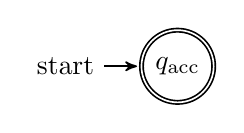
\begin{tikzpicture}[->,>=stealth',shorten >=1pt, auto, node distance=2cm, semithick]
  \tikzstyle{every state}=[text=black, fill=none]
  \node[initial,state,accepting] (q0)                    {$q_{\mathrm{acc}}$};
 ;
\end{tikzpicture}}
$, \varepsilon \rangle$}  
& \text{if } x = \langle M, w \rangle \text{ for a Turing machine $M$ and string $w$}\\
& \qquad \qquad \text{ and } w \in L(M) \\

\scalebox{.7}{$\langle$ \hspace{-.5cm} \raisebox{-.4cm}{
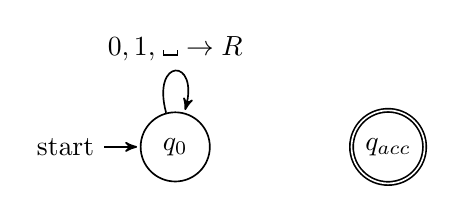
\begin{tikzpicture}[->,>=stealth',shorten >=1pt, auto, node distance=2cm, semithick]
  \tikzstyle{every state}=[text=black, fill=none]
  \node[initial,state] (q0)                    {$q_0$};
  \node[state,accepting] (qacc) [right of = q0, xshift = 20]{$q_{acc}$};
  \path (q0) edge  [loop above] node {$0, 1, \blank \to R$} (q0)
 ;
\end{tikzpicture}}
$\rangle$} 
& \text{otherwise}
\end{cases} 
\]


\item\gradeComplete $A_{\mathrm{TM}} \le_m EQ_{\mathrm{TM}} $ with 
\[
f(x) = \begin{cases}
 \scalebox{.7}{$\langle$ \hspace{-.5cm} \raisebox{-.4cm}{
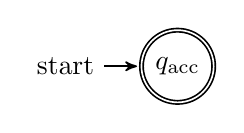
\begin{tikzpicture}[->,>=stealth',shorten >=1pt, auto, node distance=2cm, semithick]
  \tikzstyle{every state}=[text=black, fill=none]
  \node[initial,state,accepting] (q0)                    {$q_{\mathrm{acc}}$};
 ;
\end{tikzpicture}}
, $M_w \rangle$}  & \text{if } x = \langle M, w \rangle \text{ for a Turing machine $M$ and string $w$}\\\\
\scalebox{.7}{$\langle$ \hspace{-.5cm} \raisebox{-.4cm}{
    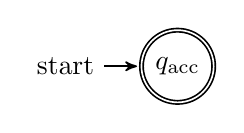
\begin{tikzpicture}[->,>=stealth',shorten >=1pt, auto, node distance=2cm, semithick]
      \tikzstyle{every state}=[text=black, fill=none]
      \node[initial,state,accepting] (q0)                    {$q_{\mathrm{acc}}$};
     ;
    \end{tikzpicture}}}
    , ~~~
    \scalebox{.7}{\hspace{-.5cm} \raisebox{-.4cm}{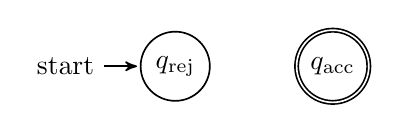
\begin{tikzpicture}[->,>=stealth',shorten >=1pt, auto, node distance=2cm, semithick]
        \tikzstyle{every state}=[text=black, fill=none]
        \node[initial,state] (qrej)                    {$q_{\mathrm{rej}}$};
        \node[state,accepting] (qacc) [right of=qrej]            {$q_{\mathrm{acc}}$};
       ;
      \end{tikzpicture}}$\rangle$ }  & \text{otherwise}.
\end{cases}
\]
Where for each Turing machine $M$, we  define 
\begin{align*}
    M_w = ``&\text{On input } y \\
    &1. \text{   Simulate $M$ on $w$.}\\
    &2. \text{   If it accepts, accept.}\\
    &3. \text{   If it rejects, reject."}
\end{align*}

\item\gradeCorrectFirst $HALT_{\mathrm{TM}} \le_m EQ_{\mathrm{TM}} $ with 
\[
f(x) = \begin{cases}
 \scalebox{.7}{$\langle$ \hspace{-.5cm} \raisebox{-.4cm}{
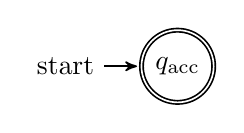
\begin{tikzpicture}[->,>=stealth',shorten >=1pt, auto, node distance=2cm, semithick]
  \tikzstyle{every state}=[text=black, fill=none]
  \node[initial,state,accepting] (q0)                    {$q_{\mathrm{acc}}$};
 ;
\end{tikzpicture}}
, $M_w \rangle$}  & \text{if } x = \langle M, w \rangle \text{ for a Turing machine $M$ and string $w$}\\\\
\scalebox{.7}{$\langle$ \hspace{-.5cm} \raisebox{-.4cm}{
    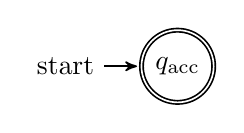
\begin{tikzpicture}[->,>=stealth',shorten >=1pt, auto, node distance=2cm, semithick]
      \tikzstyle{every state}=[text=black, fill=none]
      \node[initial,state,accepting] (q0)                    {$q_{\mathrm{acc}}$};
     ;
    \end{tikzpicture}}}
    , ~~~
    \scalebox{.7}{\hspace{-.5cm} \raisebox{-.4cm}{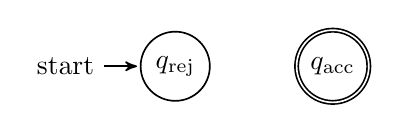
\begin{tikzpicture}[->,>=stealth',shorten >=1pt, auto, node distance=2cm, semithick]
        \tikzstyle{every state}=[text=black, fill=none]
        \node[initial,state] (qrej)                    {$q_{\mathrm{rej}}$};
        \node[state,accepting] (qacc) [right of=qrej]            {$q_{\mathrm{acc}}$};
       ;
      \end{tikzpicture}}$\rangle$ }  & \text{otherwise}.
\end{cases}
\]
Where for each Turing machine $M$, we  define 
\begin{align*}
    M_w = ``&\text{On input } y \\
    &1. \text{   If } y \text{ is not the empty string, reject.}\\
    &2. \text{   Else, simulate $M$ on $w$.}\\
    &3. \text{   If it accepts, accept.}\\
    &4. \text{   If it rejects, reject."}
\end{align*}

\item\gradeCorrect $\{w w \mid w \in \{0,1\}^* \} \leq \emptyset$ and
$f(x) = 1$ for each $x \in \{0,1\}^*$.

\item\gradeCorrect $\emptyset \le_m \{w w \mid w \in \{0,1\}^* \}$ and
$f(x) = 1$ for each $x \in \{0,1\}^*$.


\end{enumerate}

%%%%%%%%%%% PROBLEM 2 %%%%%%%%%%%
\item\textbf{Using mapping reductions} (14 points):
Consider the following computational problems we've discussed
\begin{align*}
A_{TM} &= \{ \langle M, w \rangle \mid M \text{ is a Turing machine, } w \text{ is a string and $M$ accepts $w$}\} \\
HALT_{TM} &= \{ \langle M, w \rangle \mid M \text{ is a Turing machine, } w \text{ is a string and $M$ halts on $w$}\} \\
E_{TM} &=  \{ \langle M \rangle \mid M \text{ is a Turing machine and } L(M) = \emptyset\} \\
EQ_{TM} &= \{ \langle M_1, M_2 \rangle \mid M_1, M_2 \text{ are both Turing machines and } L(M_1) = L(M_2) \}
\end{align*}
and the new computational problem
\[
    Two_{TM} = \{ \langle M \rangle \mid M \text{ is a Turing machine and $M$ accepts exactly one string} \}
\]

\begin{enumerate}
\item[(a)] \gradeCorrect Give an example of a string that is an element of $Two_{TM}$ and a string that is not an element of
$Two_{TM}$ and briefly justify your choices.
\item[(b)] \gradeComplete Prove that $Two_{TM}$ is not decidable by showing that $A_{TM} \leq_m Two_{TM}$.
\item[(c)] \gradeCorrect Give a different proof that $Two_{TM}$ is not decidable by showing that $HALT_{TM} \leq_m Two_{TM}$.
\item[(d)] \gradeComplete Is $Two_{TM}$ recognizable? Justify your answer.
\end{enumerate}

%%%%%%%%%%% PROBLEM 3 %%%%%%%%%%%
\item\textbf{Using mapping reductions} (14 points):
Consider the following computational problems we've discussed
\begin{align*}
A_{TM} &= \{ \langle M, w \rangle \mid M \text{ is a Turing machine, } w \text{ is a string and $M$ accepts $w$}\} \\
HALT_{TM} &= \{ \langle M, w \rangle \mid M \text{ is a Turing machine, } w \text{ is a string and $M$ halts on $w$}\} \\
E_{TM} &=  \{ \langle M \rangle \mid M \text{ is a Turing machine and } L(M) = \emptyset\} \\
EQ_{TM} &= \{ \langle M_1, M_2 \rangle \mid M_1, M_2 \text{ are both Turing machines and } L(M_1) = L(M_2) \}
\end{align*}
and the new computational problem
\begin{align*}
    Evens_{TM} &= \{ \langle M \rangle \mid M \text{ is a Turing machine 
    and any string that $M$ accepts must be even length}\\
    &\text{(but there may even length strings that $M$ doesn't accept)} \}
\end{align*}
\begin{enumerate}
\item[(a)] \gradeCorrect Give an example of a string that is an element of $Evens_{TM}$ and a string that is not an element of
$Evens_{TM}$ and briefly justify your choices.
\item[(b)] \gradeComplete Prove that $Evens_{TM}$ is not decidable by showing that $HALT_{TM} \leq_m Evens_{TM}$.
\item[(c)] \gradeCorrect Give a different proof that $Evens_{TM}$ is not decidable by showing that $A_{TM} \leq_m Evens_{TM}$.
\item[(d)] \gradeComplete Is $Evens_{TM}$ recognizable? Justify your answer.
\end{enumerate}


%%%%%%%%%%% PROBLEM 4 %%%%%%%%%%%
\item \textbf{Examples of languages} (7 points):

For each part of the question, use precise mathematical notation or English to define your examples
and then briefly justify why they work.

\begin{enumerate}
    \item\gradeCorrect Two undecidable languages $L_1$ and $L_2$ over the same alphabet
        whose intersection $L_1 \cap L_2$ is decidable, or write {\bf NONE}
        if there is no such example (and explain why).
    
    \item\gradeCorrect A regular language $L_3$ and an unrecognizable
        language $L_4$ over the same alphabet whose set-wise concatenation $L_3 \circ L_4$ is unrecognizable, 
        or write {\bf NONE} if there is no such example (and explain why).
    
    
    \item\gradeComplete A co-recognizable language $L_5$ that is NP-complete,
         or write {\bf NONE} if there is no such example (and explain why).
        Recall the definition: A language $L$ over an  alphabet $\Sigma$ is called {\bf co-recognizable} if its complement,  defined
        as $\Sigma^* \setminus L  = \{ x  \in  \Sigma^* \mid x \notin  L \}$, is Turing-recognizable.
        
\end{enumerate}
    

\end{enumerate}
\end{document}